\documentclass[11pt]{exam}
\pagestyle{headandfoot}
\firstpageheader{}{}{}
\runningheader{\date}{}{\class, \teacher}
\runningheadrule
\firstpagefooter{}{}{}
\runningfooter{}{Viel Erfolg!}{Seite \thepage\:von \numpages}
\runningfootrule
%=========================================================
\newcommand{\theme}{Trigonometrie}
\newcommand{\teacher}{Jonas Guler}
\newcommand{\class}{2Na}
\newcommand{\serie}{Wiederholungsprüfung}
%\newcommand{\date}{\today}
\newcommand{\duration}{45 Minuten}
\newcommand{\name}{\bf Name:}
\newcommand{\grade}{Note:}
\newcommand{\datum}{05.04.24}
%=========================================================
\begin{document}
\fontsize{14}{14}\selectfont
%========================================================

%========================================================
\begin{tabular*}{\textwidth}{l @{\extracolsep{55mm}}l @{\extracolsep{6pt}}l}
    \textbf{\theme} & \textbf{\grade} & {\answerbox}\\
    \textbf{Klasse \class} & & \\
    \textbf{\teacher}  & {\name} &\textbf{\hrulefill}\\[8pt]
\end{tabular*}
%--------------------
\begin{center}
\rule[1ex]{\textwidth}{1pt}
Dauer: \duration \hspace{9cm}Datum: \datum\\
\vspace{5pt}
\rule[2ex]{\textwidth}{1pt}
\end{center}
%=========================================================

%=========================================================
\begin{center}
\textbf{Bewertungstabelle}\\
\small Wird von der Lehrperson ausgefüllt\\
\vspace{5pt}
\addpoints
\gradetable[h][questions]\\
\vspace{5pt}
Der Rechenweg muss \textbf{vollständig und nachvollziehbar} sein.\\
Lösen Sie die Prüfung mit einen schwarzen oder blauen Kugelschreiber. Resultate in Bleistift, roter oder grüner Farbe werden nicht berücksichtigt.\\
Die Schlussresultate sind vollständig gekürzt oder auf 3 Nachkommastellen genau anzugeben.\\
Als Hilfsmittel ist ein Tascherechner erlaubt. Kennzeichne in deinem Lösungsweg klar, wo du den Taschenrechner zur Hilfe genommen hast.
\end{center}

\noindent
\rule[1ex]{\textwidth}{1pt}

\vfill
\begin{center}
    \Huge{\serie}
\end{center}

\newpage
\begin{questions}
%=========================================================
%-------------------TESTFRAGEN
%=========================================================
\question[5] %Rhyn S2 A9f
\begin{minipage}{0.6\linewidth}
    Berechne alle fehlenden Seiten und Winkel, wenn
    \[c=7.68\quad\text{ und }\quad\alpha=3\beta\]
    gegeben sind.
\end{minipage}
\hfill
\begin{minipage}{0.35\linewidth}
    \centering
\includegraphics[scale=0.6]{Trigonometrie/data-trigo/Dreieck-Trigo.png}
\end{minipage}
\vspace{5pt}
\antwort{20}


%---------------------------------------------------------
\newpage
\question[5] % Funktionsgraphen
\textbf{Beachte:} Lösungswege mit Hilfe des Taschenrechners geben keine Punkte!
\begin{parts} 
    \part Zeichne den Winkel $\alpha=-65^\circ$ im Einheitskreis ein und gib den Sinus-, Cosinus- und Tangenswert von $\alpha$ an. 
\end{parts}
\vspace{5pt}
\begin{figure}[ht]
    \begin{tikzpicture}[cross/.style={draw, cross out, minimum size=2*(#1-1pt), inner sep=0pt, outer sep=0pt}, x=10mm, y=10mm, 
        >=latex,   %Voreinstellung für Pfeilspitzen
        font= \footnotesize, scale=3]
        %Raster zeichnen
        % \draw [color=gray!50]  [step=7.5mm] (-1.3,-5.3) grid (14.8,5.8);
        % Achsen zeichnen
        \draw[->,thick] (-1.1,0) -- (1.2,0) node[right, below] {\normalsize $x$};
        \draw[->,thick] (0,-1.1) -- (0,1.2) node[above, left] {\normalsize $y$};
        % Achsen beschriften
        \foreach \x in {-1,1} \draw (\x,-.1) -- (\x,.1) node[below=4pt] {$\x$};
        \foreach \y in {-1,1} \draw (-.1,\y) -- (.1,\y) node[left=4pt] {$\y$};
        % Besserer Ursprung
        \draw[color=black] (0pt,-3pt) node[right] {$0$};
        %Funktionen zeichnen:
        \clip(-1.1,-1.1) rectangle (1.1,1.1); %Bildbereich
        \draw circle [radius=1];
    \end{tikzpicture}
\end{figure}
\begin{parts} 
    \setcounter{partno}{1}
    \part Berechne alle Winkel $\beta$ zwischen $0^\circ$ und $360^\circ$ für welche gilt: \[\tan{\beta}=-2\]
\end{parts}
\begin{figure}[ht]
    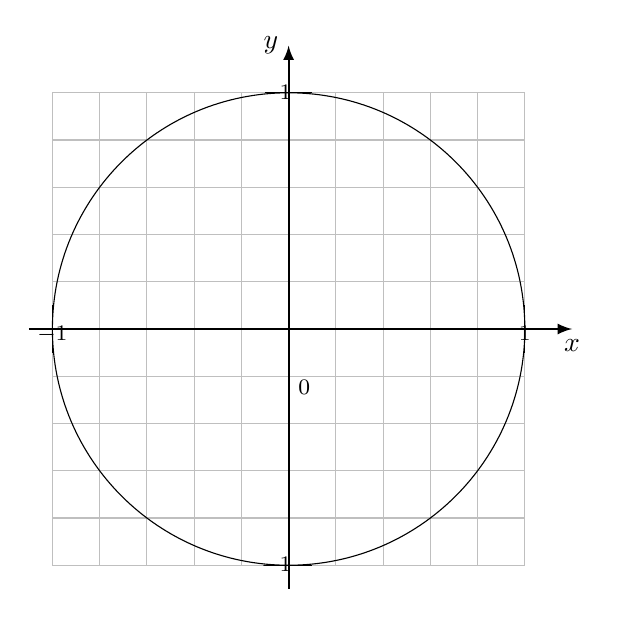
\begin{tikzpicture}[cross/.style={draw, cross out, minimum size=2*(#1-1pt), inner sep=0pt, outer sep=0pt}, x=10mm, y=10mm, 
        >=latex,   %Voreinstellung für Pfeilspitzen
        font= \footnotesize, scale=3]
        %Raster zeichnen
        \draw [color=gray!50]  [step=2mm] (-1,-1) grid (1,1);
        % Achsen zeichnen
        \draw[->,thick] (-1.1,0) -- (1.2,0) node[right, below] {\normalsize $x$};
        \draw[->,thick] (0,-1.1) -- (0,1.2) node[above, left] {\normalsize $y$};
        % Achsen beschriften
        \foreach \x in {-1,1} \draw (\x,-.1) -- (\x,.1) node[below=4pt] {$\x$};
        \foreach \y in {-1,1} \draw (-.1,\y) -- (.1,\y) node[left=4pt] {$\y$};
        % Besserer Ursprung
        \draw[color=black] (0pt,-7pt) node[right] {$0$};
        %Funktionen zeichnen:
        \clip(-1.1,-1.1) rectangle (1.1,1.1); %Bildbereich
        \draw circle [radius=1];
    \end{tikzpicture}
\end{figure}


%---------------------------------------------------------
\newpage
\question[4] %GZP 13 A8
Berechne in der folgenden Figur den Winkel $\phi$.
\begin{figure}[ht]
    \centering
\includegraphics[scale=1]{Trigonometrie/data-trigo/ThalesÄhnlichkeit.png}
\end{figure}
\vspace{5pt}
\antwort{16}


%---------------------------------------------------------
\newpage
\question[4] % GZP 16 A12
\begin{parts}
    \part Berechne \[\oldcos^2(\alpha)\*\tan{\alpha}-\oldsin^2(\alpha)\*\frac{1}{\tan{\alpha}}\]
\end{parts}
\vspace{5pt}
\antwort{8}
\begin{parts}
    \setcounter{partno}{1}
    \part Entscheide, ob die Aussagen in der Tabelle unten wahr oder falsch sind. Die Antworten müssen nicht begründet werden.\newline
    \begin{small}
        Bewertung: Für $0-2$ richtige Antworten gibt es keine Punkte, $3$ richtige Antworten einen Punkt und falls alle Antworten richtig sind, gibt es $2$ Punkte.
    \end{small}
    \begin{table}[h]
        \centering
        \begin{tabular}{|p{10cm}|c|c|}\hline
             & wahr & falsch\\\hline
            $\displaystyle\sin{90^\circ-\alpha}=\sin{90^\circ+\alpha}$ &  & \\\hline
            $\displaystyle\cos{\alpha}=-\cos{-\alpha}$ &  & \\\hline
            $\displaystyle\oldsin^2(\alpha)+\oldcos^2(\alpha)=\oldtan^2(\alpha)$ &  & \\\hline
            $\displaystyle\tan{270^\circ}$ ist nicht definiert. &  & \\\hline
        \end{tabular}
    \end{table}
\end{parts}


%---------------------------------------------------------
\newpage
\question[4] %
\begin{minipage}{0.6\linewidth}
    Du siehst von zwei verschiedenen Punkten, $A$ und $B$, die Spitze des Säntis. Beide Punkte befinden sich $400$m über Meer. Die Distanz zwischen $A$ und $B$ beträgt exakt $8.1$km. Beim Punkt $A$ siehst du die Spitze unter einem Winkel $\alpha=6^\circ$ und bei $B$ gilt $\beta=10^\circ$.\vspace{5pt}
    \begin{parts}
        \part Zeige rechnerisch, dass der Säntis ca. $2500$m hoch ist.
        \part Wie nahe bist du dem Säntis vom Punkt $B$?
    \end{parts}
\end{minipage}
\hfill
\begin{minipage}{0.35\linewidth}
    \centering
\includegraphics[scale=0.6]{Trigonometrie/data-trigo/Aussichtspunkt.png}
\end{minipage}
\vspace{7pt}
\antwort{17}


%---------------------------------------------------------
\newpage
\question[4] %GZP 18 A20
Im Rechteck $ABCD$ beträgt $\overline{AD}=10$cm, $\alpha=30^\circ$ und $\beta=70^\circ$. Berechne die Strecke $\overline{CE}$.
\begin{figure}[ht]
    \centering
\includegraphics[scale=0.5]{Trigonometrie/data-trigo/RechteckStrecke.png}
\end{figure}
\vspace{5pt}
\antwort{18}
\end{questions}
\end{document}